\documentclass[11pt, twoside, BCOR=8mm, DIV=12]{scrartcl}
%\usepackage[german,ngerman]{babel}
\usepackage[utf8]{inputenc}
\usepackage[T1]{fontenc}
\usepackage{color}
\usepackage{graphicx}
\usepackage{amsmath}
\usepackage{eurosym}
\usepackage[hyphens]{url}

\usepackage[onehalfspacing]{setspace}

\usepackage{float}
\usepackage{listingsutf8}
\usepackage{booktabs}
\usepackage{enumitem}
\usepackage{pgfplots}

\title{{\Large INFORMATION VISUALIZATION, WINTER TERM 2017/18} \\ Exercise 6 – InfoVis Project Milestone 3}

\begin{document}
\maketitle
\section*{Task 1: Milestone 3 - Working Prototype}
Link to presentation: \\ \url{https://docs.google.com/presentation/d/1LXW_66N4tAOHmNkLnnxPiKmOqKrUxHCQUatqXEHj9Cg/edit?usp=sharing}
\begin{enumerate}[label=\alph*)]
\item \textbf{Running prototype} \\
At the moment we do not have a webspace available to use our prototype. Our site or framework works without any additional software products.
Just look under the project folder.

For an animated graph (Parallel Coordinates), however, we use a csv file as data source. Reading them in locally causes an error message in the common browsers (see "Cross origin requests are only supported for protocol schemes: http, data, chrome, chrome-extension, https.").
Minimizing the security of the browser and allowing loading / parsing of local files does not seem like a good solution. 
For this reason, we use a local web server (Apache web server) so that the graph can be created.

We will look for a better solution for the following milestone.

\item \textbf{Functionality}
You can visit the page.

If the page is running under a web service, the Parallel Coordinates Graph can be used. All values from the Oktoberfest.csv file are shown in this graph. On the axes, you can select between individual values, thus focusing the relationships of the data.
Unfortunately, this graph (our animation) only works under a webservice (see a)). We could not solve in time otherwise this problem regrettably.
Here are a few pictures to present the graph at this point:
\begin{figure}[H]
	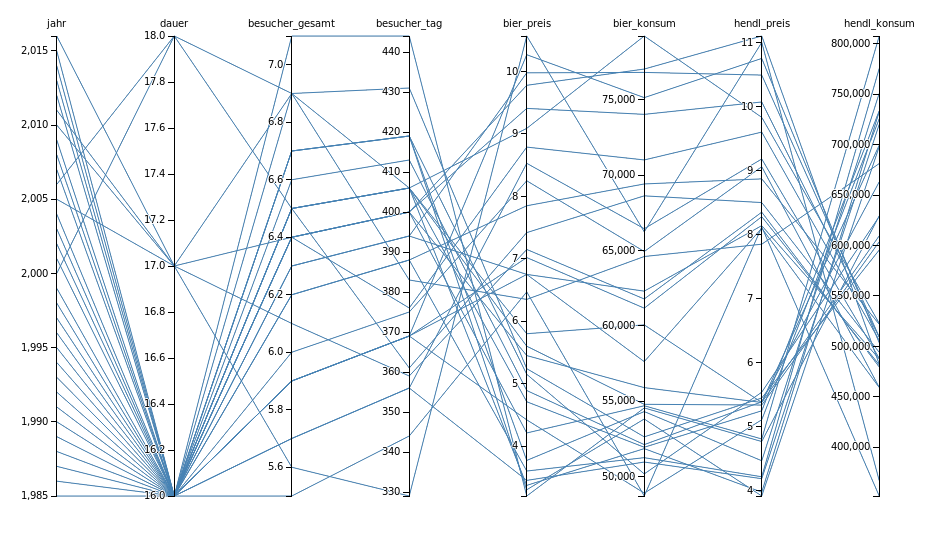
\includegraphics[width=\textwidth]{./img/parallelCoordinates_1}
	\caption{Parallel Coordiantes with any scale selection}
	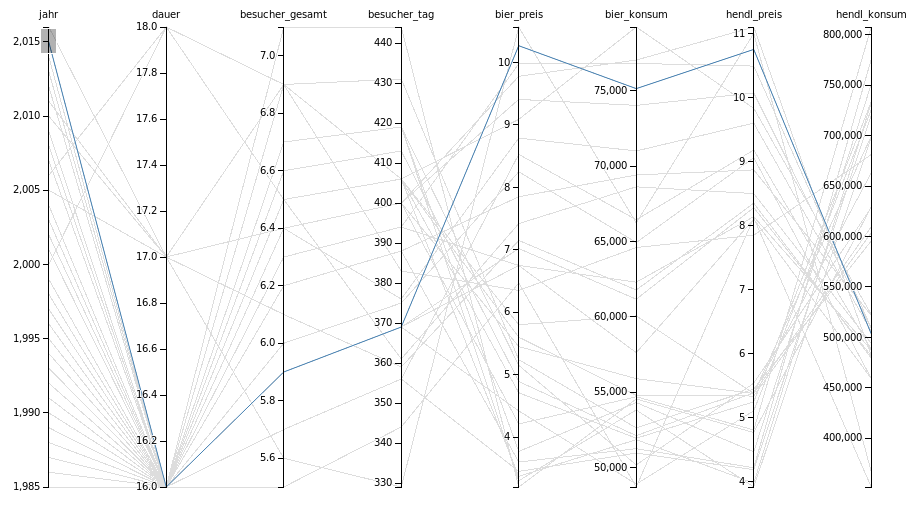
\includegraphics[width=\textwidth]{./img/parallelCoordinates_2}
	\caption{Parallel Coordiantes with scale selection for one year}
\end{figure}

\item \textbf{Roadmap} \\
Until we reach the feature set of our intended final product, we need to:
\begin{itemize}
	\item answer all (remaining) questions
	\item implementing the other graphs and animations
	\item present the data in a good context
	\item fix the problem with local csv-file (e.g. using a link to web space for our prototype or final product)
\end{itemize}
\end{enumerate}

\end{document}